% FADO --- CISUC template, Beamer version.
% Compiles with pdfLaTeX, XeLaTeX, or LuaLaTeX (run twice for the TikZ overlays).
\documentclass[aspectratio=169]{beamer}
\usepackage{geometry}
\geometry{paperwidth=13.333in,paperheight=7.5in}
\usepackage{iftex}
\usepackage{tikz}
\usetikzlibrary{arrows.meta}
\usepackage{booktabs}
\usepackage{multirow}
\usepackage{amsmath}
\usepackage{array}

% ---- fonts (engine-agnostic; TeXLive-bundled Helvetica/Courier clones, no fontspec) ----
\ifPDFTeX\usepackage[utf8]{inputenc}\fi
\usepackage[T1]{fontenc}
\usepackage{textcomp}
\usepackage{tgheros}   % Helvetica clone (Arial-like) sans
\usepackage{tgcursor}  % Courier clone mono
\renewcommand{\familydefault}{\sfdefault}
\newcommand{\monofont}{\ttfamily}

% ---- colours ----
\definecolor{cred}{HTML}{DA0725}
\definecolor{ink}{HTML}{141414}
\definecolor{body}{HTML}{262626}
\definecolor{grey}{HTML}{9A9A9A}
\definecolor{lgrey}{HTML}{C4C4C4}
\definecolor{rulec}{HTML}{2A2A2A}
\definecolor{green}{HTML}{2E9E5B}
\definecolor{amber}{HTML}{C77A18}

\setbeamercolor{normal text}{fg=body}
\setbeamercolor{itemize item}{fg=cred}
\setbeamercolor{itemize subitem}{fg=cred}
\setbeamercolor{itemize subsubitem}{fg=cred}
\setbeamercolor{enumerate item}{fg=cred}
\setbeamercolor{enumerate subitem}{fg=cred}
\setbeamercolor{enumerate subsubitem}{fg=cred}
\setbeamercolor{item projected}{fg=cred}
\setbeamertemplate{navigation symbols}{}
\setbeamersize{text margin left=0pt,text margin right=0pt}

% ---- running header (shown on non-plain frames) ----
\newcommand{\hdrsec}{}
\newcommand{\hdrpg}{}
\newcommand{\pageset}[2]{\renewcommand{\hdrsec}{#1}\renewcommand{\hdrpg}{#2}}
\setbeamertemplate{headline}{%
  \vskip3mm%
  \makebox[\paperwidth][c]{%
    \hspace{9mm}%
    \parbox[t]{4.2in}{\monofont\color{grey}\fontsize{9}{11}\selectfont
      FADO: A Reaction Controller for Fairness-\\ Aware Online Learning Under Concept Drift}%
    \hfill
    \parbox[t]{4.2in}{\centering\monofont\color{grey}\fontsize{10}{12}\selectfont \hdrsec}%
    \hfill
    \parbox[t]{2.6in}{\raggedleft\monofont\fontsize{13}{15}\selectfont
      \textbf{\color{ink}\hdrpg}{\color{grey}/12}}%
    \hspace{9mm}%
  }%
}
\setbeamertemplate{footline}{}
\setbeamertemplate{frametitle}{}

% ---- helpers (absolute placement via TikZ overlay) ----
% \tb{width-in}{x-in}{y-in}{content}  --- anchored top-left at (x,y) from page NW
% optional #1 = extra node options (use font=... for large text so spacing scales)
\newcommand{\tb}[5][]{\begin{tikzpicture}[remember picture,overlay]%
  \node[anchor=north west,inner sep=0pt,outer sep=0pt,text width=#2in,align=left,#1]
    at ([xshift=#3in,yshift=-#4in]current page.north west){\raggedright #5\par};\end{tikzpicture}}
\newcommand{\fs}[2]{\fontsize{#1}{#2}\selectfont}
\newcommand{\hrl}[3]{\tb{#3}{#1}{#2}{{\color{lgrey}\rule{#3in}{0.9pt}}}}
% square outline cell with centred label: \boxcell{x}{y}{size-in}{label}
\newcommand{\boxcell}[4]{\begin{tikzpicture}[remember picture,overlay]%
  \node[draw=lgrey,line width=0.8pt,anchor=north west,minimum width=#3in,minimum height=#3in,
    align=center,text=ink,font=\fontsize{14}{16}\selectfont]
    at ([xshift=#1in,yshift=-#2in]current page.north west){#4};\end{tikzpicture}}
% arrow from (x1,y1) to (x2,y2) in inches from page NW
\newcommand{\parrow}[4]{\begin{tikzpicture}[remember picture,overlay]%
  \draw[-{Latex[length=2mm]},line width=1.3pt,ink]
    ([xshift=#1in,yshift=-#2in]current page.north west)--([xshift=#3in,yshift=-#4in]current page.north west);\end{tikzpicture}}
% column helpers (fixed y per slide type) --- defined once, avoid in-frame defs
\newcommand{\colblk}[4]{%
  \tb{3.5}{#1}{2.45}{\bfseries\color{ink}\fs{17}{20}#2}%
  \tb{3.5}{#1}{2.9}{\itshape\color{grey}\fs{12}{14}#3}%
  \hrl{#1}{3.32}{3.3}%
  \tb{3.3}{#1}{3.5}{\color{body}\fs{13.5}{17}#4}}
\newcommand{\phaseblk}[4]{%
  \tb{3.5}{#1}{2.5}{\bfseries\color{cred}\fs{17}{20}#2}%
  \tb{3.5}{#1}{2.95}{\itshape\color{grey}\fs{13}{15}#3}%
  \hrl{#1}{3.35}{3.1}%
  \tb{3.2}{#1}{3.5}{\color{body}\fs{13}{16}#4}}
\newcommand{\dcolblk}[3]{%
  \tb{3.6}{#1}{2.55}{\bfseries\color{ink}\fs{16}{19}#2}%
  \hrl{#1}{3.35}{3.3}%
  \tb{3.4}{#1}{3.5}{\color{body}\fs{14}{18}#3}}
\newcommand{\ctitle}[1]{\tb[font=\fontsize{28}{28}\selectfont\bfseries]{11.6}{0.85}{1.4}{\color{ink}#1}}
\newcommand{\divider}[2]{\tb[font=\fontsize{40}{46}\selectfont\bfseries]{11.3}{1.0}{3.05}{%
  \centering{\color{cred}#1.\ }{\color{ink}#2}}}
\newcommand{\body}[1]{\tb{7.1}{0.85}{2.5}{\color{body}\fs{17}{23}\setlength{\parskip}{9pt}#1}}
\newcommand{\centerimage}[3]{%
  \pgfmathsetmacro{\centerimagex}{(13.333-#1)/2}%
  \tb{#1}{\centerimagex}{#2}{\includegraphics[width=#1in]{#3}}}
\newcommand{\codepanel}[3]{%
  \tb{5.45}{#1}{2.25}{\bfseries\color{cred}\fs{16}{19}#2}%
  \hrl{#1}{2.8}{5.45}%
  \tb{5.45}{#1}{3.05}{\color{body}\ttfamily\fs{10.2}{12.5}#3}}
\newcommand{\slidefoot}[1]{%
  \tb{11.6}{0.85}{6.45}{\centering\color{grey}\fs{13}{16}#1}}
\newcommand{\question}[4]{\hrl{8.35}{#1}{4.1}\tb{4.1}{8.35}{#2}{\fs{14}{18}{\color{cred}\bfseries #3}\par\smallskip{\color{ink}#4}}}
\newcommand{\outlineitem}[2]{\color{cred}\bfseries #1.\hspace{0.6em}{\color{ink}#2}\par}
\newcommand{\titleSlide}[2]{%
  \tb[font=\fontsize{46}{50}\selectfont\bfseries]{11.4}{0.9}{2.4}{\color{ink}#1}%
  \tb[font=\fontsize{30}{36}\selectfont\bfseries]{11.4}{0.9}{3.4}{\color{ink}#2}%
  \tb{2.5}{0.9}{6.75}{
\includegraphics[width=2.5in]{assets/cisuc_logo.png}}}

\begin{document}

% ===================================================== 1 LOGO
\begin{frame}[plain]
  \tb{4.6}{4.37}{3.35}{
\includegraphics[width=4.6in]{assets/cisuc_logo.png}}
\end{frame}

% ===================================================== 2 TITLE
\begin{frame}[plain]
  \titleSlide{FADO} {Meeting 2}
  \tb{11}{0.92}{4.55}{\color{ink}\fs{19}{22}Tiago Silva}
  \tb{11}{0.92}{5.35}{\color{ink}\fs{14}{18}\textbf{CISUC \textperiodcentered{} Data-Centric AI Lab}\\
    {\color{body}\fs{14}{18}Department of Informatics Engineering, University of Coimbra}}
  \tb{2.5}{0.9}{6.75}{
\includegraphics[width=2.5in]{assets/cisuc_logo.png}}
\end{frame}

% ===================================================== 3 OUTLINE (01)
\pageset{Outline}{01}
\begin{frame}
  \ctitle{Outline}
  \body{
    \begin{enumerate}
      \item \textbf{Weekly reviews}: KANs;
      \item \textbf{Review pass}: what we found, what we fixed, a correction;
      \item \textbf{Decisions taken};
      \item \textbf{The $\lambda$ controller}: the answer to the novelty critique;
      \item \textbf{First results} and how they happened;
      \item \textbf{Ablation plan}, open questions and next steps.
    \end{enumerate}
  }
\end{frame}

\pageset{Weekly reviews - KANs}{02}
\begin{frame}
    \ctitle{KANs}
    \tb{3.9}{4.72}{2.55}{
\includegraphics[width=3.9in]{assets/D3KAN.png}}
    \tb{3.9}{0.45}{2.55}{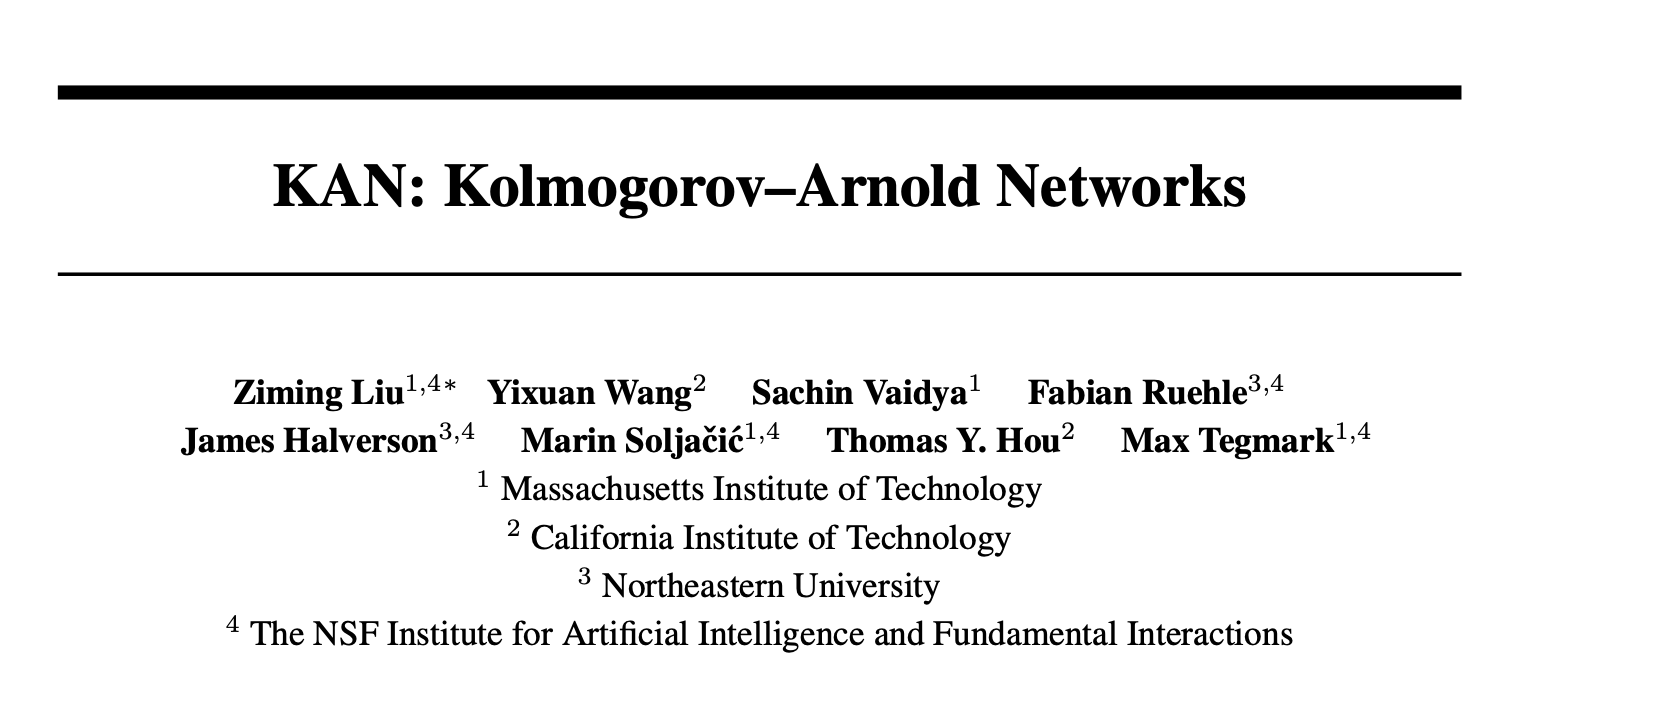
\includegraphics[width=3.9in]{assets/ClassicKAN.png}}
    \tb{3.9}{8.99}{2.55}{
\includegraphics[width=3.9in]{assets/fairKAN.png}}
    \tb[align=center]{3.9}{0.45}{4.35}{\color{body}\fs{12}{14}\textbf{Kolmogorov-Arnold Networks}\par\smallskip
      Activation functions are placed on edges instead of nodes.}
    \tb[align=center]{3.9}{4.72}{4.35}{\color{body}\fs{12}{14}\textbf{$D^3$KAN}\par\smallskip
      A denoising and data-complexity-adaptive KAN for long-term forecasting.}
    \tb[align=center]{3.9}{8.99}{4.35}{\color{body}\fs{12}{14}\textbf{Learning Fair Representations with KANs}\par\smallskip
      KANs applied to learning fair representations.}
\end{frame}

% ===================================================== REVIEW PASS (03)
\pageset{Review pass}{03}
\begin{frame}
  \ctitle{The review pass: results we {\color{cred}\textit{\underline{could not}}} trust}
  \dcolblk{0.85}{Invalid results}{%
    COMPAS loader cut every split to \textbf{10 rows}: every stored COMPAS number came from 10 test samples.\\[5pt]
    Significance script turned untestable comparisons ($n<2$) into $p=0$, \textbf{***}.
  }
  \dcolblk{4.85}{Silently inert experiments}{%
    COMPAS defaults overwrote the swept flags: every cell of the old sensitivity sweep ran \textbf{one} configuration.\\[5pt]
    The W\&B summary crashed before writing the metric the sweeps optimise.
  }
  \dcolblk{8.85}{Arms not comparable}{%
    On COMPAS, FADO/Base used a 250-sample window, ARF/RFR 1000.\\[5pt]
    Pre-training used $\lambda=0.1$, evaluation $\lambda=1.0$.\\[5pt]
    All fixed; COMPAS must be \textbf{re-run}.
  }
  \slidefoot{Checked and fine: no stored run hit the variable-dispatch collision ($d$ = 108, 19, 760 vs $2^{\text{depth}}$).}
\end{frame}

% ===================================================== CORRECTION (04)
\pageset{Review pass}{04}
\begin{frame}
  \ctitle{A {\color{cred}\textit{\underline{correction}}} to Meeting 1}
  \body{
    \textbf{``37.12 $\rightarrow$ 13.22 minutes on Adult''} timed a benchmark copy of the recursive updater, \textbf{not the code the pipeline ran}.\par
    The production path is now the level-wise vectorised updater, chosen by depth (\texttt{'auto'}).\par
    The benchmark will be rewritten to time the production forest, and the headline number replaced.
  }
  \slidefoot{The complexity argument, $O(B\times4^n)\rightarrow O(B\times2^n)$, stands; the wall-clock figure does not until re-measured.}
\end{frame}

% ===================================================== DECISIONS (05)
\pageset{Decisions}{05}
\begin{frame}
  \ctitle{Decisions taken}
  \tb{11.6}{0.85}{2.3}{\color{body}\fs{16}{21}
    \begin{tabular}{@{}p{2.6in}p{8.6in}@{}}
      \toprule
      \textbf{Scope} & Exclusively online learning. \\
      \textbf{$\lambda$ comparison} & Report accuracy-vs-DP \textbf{trade-off curves} over one shared $\lambda$ grid; no $\lambda$ is picked. \\
      \textbf{Tuning budget} & Controller ablations vary only the controller; parameters that reach every arm ($\lambda$, depth, trees, windows) are swept for every arm. \\
      \textbf{Metrics} & Whole-stream \textbf{and} per-phase / post-drift accuracy and DP. \\
      \textbf{Search} & Grid for factorials, random for sensitivity; report distributions, never an argmax. \\
      \textbf{Seeds} & Tune on 11--55, report on 66--202. COMPAS splits by seed only (two scenarios). \\
      \textbf{Per-tree $\lambda$} & Deferred; at most an ablation. \\
      \bottomrule
    \end{tabular}}
\end{frame}

% ===================================================== LAMBDA CONTROLLER (06)
\pageset{The $\lambda$ controller}{06}
\begin{frame}
  \ctitle{Answering {\color{cred}\textit{\underline{novelty}}}: $\lambda$ becomes a dual variable}
  \dcolblk{0.85}{Constraint}{%
    DP $=\max_g|D_g|$, with $D_g$ the gap between group $g$ and the mean positive rate.\\[5pt]
    Target: $+D_g\le\varepsilon$ and $-D_g\le\varepsilon$ for every $g$.
  }
  \dcolblk{4.85}{Signal}{%
    One sample gives $v_t[g]$ with $\mathbb{E}[v_t[g]]=D_g$ (Horvitz--Thompson).\\[5pt]
    Unbiased, no window, no autocorrelation.
  }
  \dcolblk{8.85}{Update, every sample}{%
    $\mu\leftarrow\mathrm{clip}(\mu+\eta(\pm v_t[g]-\varepsilon),\,0,\,\lambda_{\max})$\\[5pt]
    $\lambda_t=\min(\lambda_{\text{base}}+\textstyle\sum\mu,\ \lambda_{\max})$
  }
  \slidefoot{Plus forgetting: every confirmed drift resets the penalty's statistics, so $\lambda$ scales a \emph{post}-drift gradient.}
\end{frame}

% ===================================================== WHY THIS SIGNAL (07)
\pageset{The $\lambda$ controller}{07}
\begin{frame}
  \ctitle{Why not feed the rolling DP?}
  \tb{6.4}{0.85}{2.4}{\color{body}\fs{14}{18}
    Stationary 50k stream: every alarm is false.\par\medskip
    \begin{tabular}{@{}lrr@{}}
      \toprule
      signal & lag-1 autocorr. & alarms, $\delta{=}10^{-5}$ \\
      \midrule
      per-sample estimate & $-0.001$ & \textbf{0} \\
      rolling DP, $W{=}250$ & $0.991$ & {\color{cred}\textbf{24}} \\
      DP every $W$ samples & $-0.044$ & 0 \\
      \bottomrule
    \end{tabular}}
  \tb{4.9}{7.6}{2.4}{\color{body}\fs{15}{20}
    Detectors assume independent inputs; a rolling DP shares $W{-}1$ of $W$ samples with its predecessor.\par\medskip
    The per-sample estimate keeps both the detector's bound and an \textbf{unbiased} constraint gradient.}
  \slidefoot{Limits: soft trees are non-convex, so primal--dual bounds are motivation, not a guarantee.}
\end{frame}

% ===================================================== RESULTS (08)
\pageset{First results}{08}
\begin{frame}
  \ctitle{First results: DP {\color{cred}\textit{\underline{held down}}} after the drift}
  \tb{7.0}{0.85}{2.3}{\color{body}\fs{15}{20}%
    COMPAS \texttt{abrupt\_race}, 3 tuning seeds, $\lambda_{\text{base}}=0.3$, $\varepsilon=0.05$.\par\medskip
    \begin{tabular}{@{}lrrr@{}}
      \toprule
      arm & accuracy & DP & post-drift DP \\
      \midrule
      \textbf{FADO} ($\lambda$ controller) & 0.605 & \textbf{0.058} & \textbf{0.066} \\
      FADO, no reset & 0.606 & 0.081 & 0.099 \\
      FADO, $\lambda$ fixed & 0.605 & 0.094 & 0.117 \\
      Aranyani-Base & 0.617 & 0.093 & 0.116 \\
      \bottomrule
    \end{tabular}}
  \tb{4.3}{8.35}{2.3}{\color{body}\fs{14}{18}%
    \textbf{Same direction on every seed:} $-54\%$, $-18\%$, $-40\%$ DP vs.\ $\lambda$ fixed.\par\medskip
    \textbf{No accuracy cost:} ${\sim}12\%$ of predictions change; half become right, half wrong. Borderline cases move.\par\medskip
    \textbf{Not a collapse:} positive rate $0.40\rightarrow0.37$.}
  \slidefoot{A fair classifier still shows rolling DP $\approx0.026$ (window noise). 3 seeds, one scenario: a direction, not a claim.}
\end{frame}

% ===================================================== TRAJECTORY (09)
\pageset{First results}{09}
\begin{frame}
  \ctitle{How it happened: the price rises {\color{cred}\textit{\underline{while}}} DP is above target}
  \centerimage{8.1}{1.95}{assets/lambda_trajectory.png}
  \slidefoot{Identical until the drift; then the fixed-$\lambda$ arms sit at DP 0.15--0.20 while $\lambda$ climbs to 2 and holds FADO near $\varepsilon$.}
\end{frame}

% ===================================================== ABLATION PLAN (10)
\pageset{Ablation plan}{10}
\begin{frame}
  \ctitle{Ablation plan: nine sweeps, {\color{cred}\textit{\underline{ready}}} to run}
  \tb{11.6}{0.85}{2.3}{\color{body}\fs{16}{21}
    \begin{tabular}{@{}p{3.1in}p{6.3in}r@{}}
      \toprule
      \textbf{sweep} & \textbf{question} & \textbf{runs} \\
      \midrule
      component (COMPAS / Adult) & Does each part contribute? 9 presets, incl. \emph{no-$\lambda$}, \emph{$\lambda$-only}, \emph{no-reset} & 18 / 27 \\
      monitor & Which signal and detector should watch fairness? & 48 \\
      sensitivity & Basin or knife edge? Controller parameters, incl. $\varepsilon$, $\eta$ & 120 \\
      $\lambda$ budget (COMPAS / Adult) & Trade-off curves, same $\lambda$ grid for FADO and Base & 14 / 21 \\
      reference (COMPAS / Adult) & ARF / RFR points on those curves & 2 / 3 \\
      architecture & Does the gap survive other depths and tree counts? & 15 \\
      \bottomrule
    \end{tabular}}
  \slidefoot{5 tuning seeds per run; every config is validated before launch.}
\end{frame}

% ===================================================== OPEN QUESTIONS (11)
\pageset{Open questions}{11}
\begin{frame}
  \ctitle{Open questions}
  \body{
    \begin{itemize}
      \item \textbf{Target $\varepsilon$}: chosen per dataset on tuning seeds, or stated as a requirement?
      \item \textbf{Claim}: ``after drift, FADO spends fewer samples above $\varepsilon$ than Base''?
      \item \textbf{Theory}: a stability argument for non-convex soft trees, or state the convex-only caveat?
      \item \textbf{Tuning protocol}: disjoint streams, or prefix tuning (drift starts at 15--30\%, so a prefix sees none)?
      \item \textbf{Accuracy gap to Base}: comes from the LR/temperature reaction, not from $\lambda$.
    \end{itemize}
  }
\end{frame}

% ===================================================== NEXT STEPS (12)
\pageset{Next steps}{12}
\begin{frame}
  \ctitle{Next steps}
  \body{
    \begin{enumerate}
      \item Re-run COMPAS on full splits;
      \item Launch the sweeps on the tuning seeds;
      \item Metric for the claim: samples above $\varepsilon$ after each change point;
      \item Re-benchmark the production forest;
      \item Final protocol: 20 reporting seeds, all datasets, all arms.
    \end{enumerate}
  }
\end{frame}

\end{document}
